%%%%%%%%%%%%%%%%%%%%%% IDEAS SECTIOn %%%%%%%%%%%%%%%%%%
\section{Paper Intuition}
%\section{The Idea}
\label{sec:idea}

\subsection{The Problem}
\label{subsec:problem}

We address the problem of recovering from false routing state in distance vector routing.
We assume nodes are compromised such that they declare false routes to all other nodes in the network. 
{\footnote {\small  For simplicity, in this section we present our recovery algorithms in the case of a single compromised node.  The necessary extensions to handle multiple compromised nodes are 
 addressed in our Technical Report \cite{Tech}.}}
This false state spreads through the network through the normal execution of distance vector, leading to erroneous least cost paths.  We assume that the identity of the 
compromised node is provided by a different algorithm \cite{Arini,Feam,Vishal02,Pad03,Paul02}, and thus do not consider this problem in this paper.
Instead, we focus on recovering after receiving notification that a node is compromised.  The goal is for all nodes to recover correctly: each node  should 
remove the compromised node as a destination and find new least cost distances that do not use a compromised node. 
{\footnote {\small If the network becomes disconnected as a result of removing the compromised node, all nodes need only compute new least cost distances to all other nodes 
within their connected component. }}



Consider the example graph, $G$, in Figure \ref{fig:example}. Figure \ref{fig:example-a} shows $G$ before \bad is compromised. 
{\footnote {\small For convenience, we refer to \bad as the generic compromised node in the remainder of the document.}}
At this point, all least costs are correctly computed.
 {\footnote {\small Node $i$ and $j$'s routing table are shown to the right of $G$.  The least costs are underlined.}}
Now, let \bad be compromised such that it falsely declares a cost of $1$ to every other node.  Consistent with ``good news travels fast'', these false paths spread through the network,
leading to erroneous least cost paths.  For example, 
Figure \ref{fig:example-b} depicts the state of $G$ after \bads's false routing state has propagated throughout the network.  
$i$ routes via \bad to reach nodes $l$ and $d$.  $j$ uses $i$ to reach all nodes except $l$, which implies $j$ transitively uses \bad to reach these destinations 
(e.g., $j$ uses the path $j-i-\overline{v}$ then the false path from \bad to the destination). Upon receiving notification that \bad is compromised, the goal of the 
recovery is to reach the state depicted in Figure \ref{fig:example-c}: \bad is removed as a destination and no least cost uses \bad as an intermediate node. 


%Consider the example graph, $G$, in Figure \ref{fig:example}. Figure \ref{fig:example-a} shows $G$ before any nodes are compromised. All least costs are correctly computed and
%parts of node $i$ and $j$'s routing table are shown to the right of $G$.  The least costs are underlined.  Now, let \bad be compromised such that it falsely declares a cost of $1$
%to every other node.  Consistent with ``good news travels fast'', these false paths spread through the network, leading to erroneous least cost paths.  For example, 
%Figure \ref{fig:example-b} depicts the state of $G$ after \bads's false routing state has propagated throughout the network.  
%$i$ routes via \bad to reach nodes $l$ and $d$.  $j$ uses $i$ to reach all nodes except $l$.  Notice that when $j$ uses $i$ to reach $d$, it transitively uses \bad 
%(e.g., uses path $j-i-$\bads$-d$ to $d$). 

%In our problem setting, we assume an outside algorithm \cite{Arini,Feam,Vishal02,Pad03,Paul02} identifies the compromised node: in this case, \bads. From this point, the goal of the 
%recovery is to reach the state depicted in Figure \ref{fig:example-c}: \bad is removed as a destination and no least cost uses \bad as an intermediate node. 


\begin{figure*}[t]
  \begin{center}
    \subfigure[Before \bad is compromised.]{\label{fig:example-a}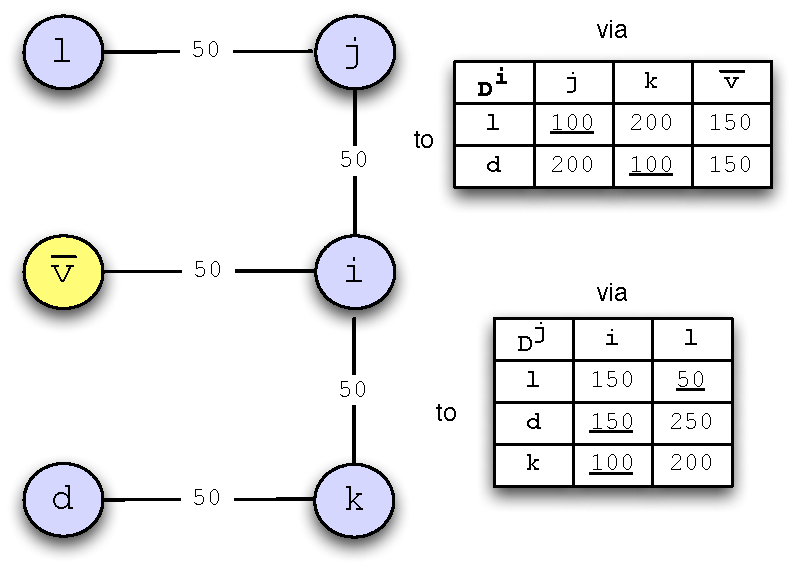
\includegraphics[scale=0.43]{figs/example-a-color.pdf}}
    \subfigure[After \bad is compromised.]{\label{fig:example-b}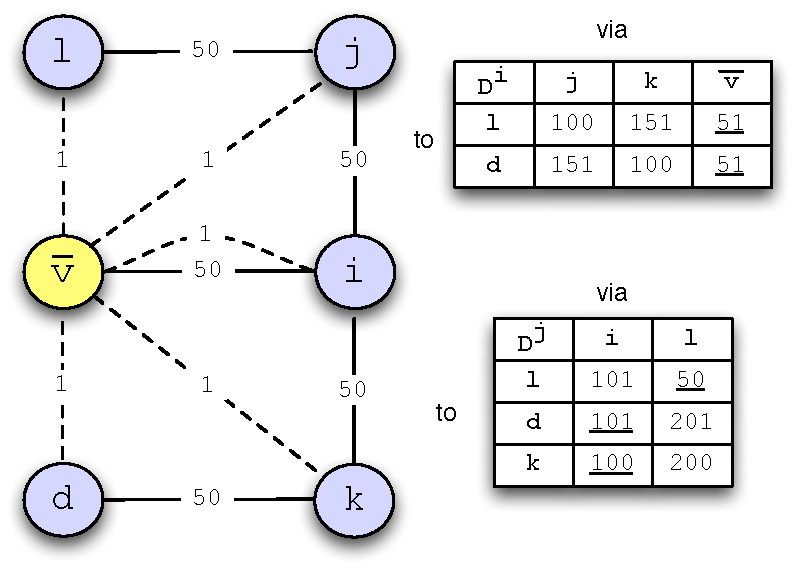
\includegraphics[scale=0.43]{figs/example-b-color.pdf}} 
    \subfigure[After recovery.]{\label{fig:example-c}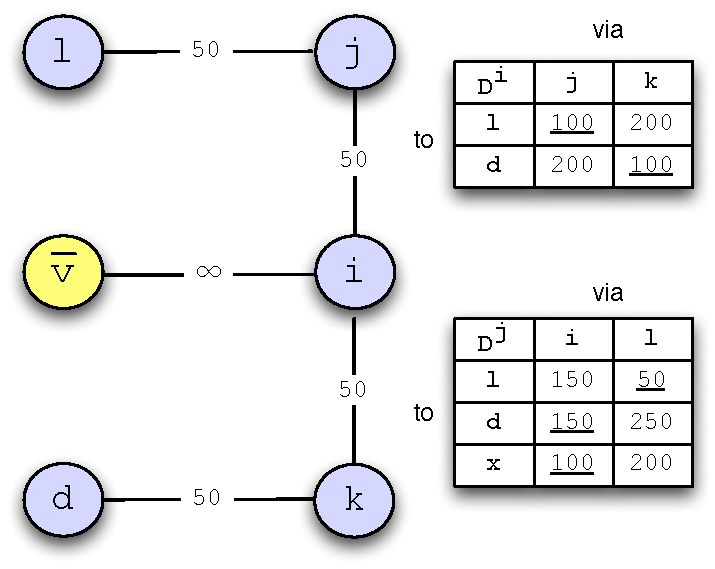
\includegraphics[scale=0.43]{figs/example-c-color.pdf}}
  \end{center}
	\caption{Three snapshots of a graph, $G$, where \bad is the compromised node: (a) $G$ before \bad is compromised, (b) $G$ after false state has 
	finished propagating but before recovery has started, and (c) $G$ after recovery. The dashed lines in (b) mark false paths. Portions of node $i$'s and $j$'s 
	routing table are displayed to the right of each sub-figure. The least cost values are underlined.}
  \label{fig:example}
\end{figure*}


\subsection{Our Solutions}
\label{subsec:algs}

In this section we propose three new recovery algorithms: \seconds, \purges, and \cprs.  The input and output of each algorithm is the same.  The input for each
algorithm is an undirected graph, correctly computed least cost paths to all nodes, and the identity of the compromised node.  The output of each 
algorithm is a new undirected graph with the compromised node removed and new least cost paths that route around the compromised node. 

First we describe a preprocessing procedure common to all three recovery algorithms. Then we describe each recovery algorithm.

\subsubsection{Preprocessing Procedure}
\label{subsubsec:preprocess}
	
All three recovery algorithms share a common preprocessing procedure.  The procedure removes the compromised node as a destination and finds the node IDs in each connected component. 
This is implemented using diffusing computations \cite{Dijkstra80} initiated at each neighbor of the compromised node. A diffusing computation is a distributed algorithm started at a source
node which grows by sending queries along a spanning tree, constructed
simultaneously as the queries propagate through the network.  When the computation reaches the leaves
of the spanning tree, replies travel back along the tree towards the
source, causing the tree to shrink. The computation eventually terminates when the
source receives replies from each of its children in the tree. 

Consider the example in Figure \ref{fig:example} where \bad is the compromised node. 
When $i$ receives the notification that \bad has been compromised, $i$ removes \bad as a destination and then initiates a diffusing computation. 
$i$ creates a vector and adds its node ID to the vector. $i$ sends a message containing this vector to $j$ and $k$.  Upon receiving $i$'s message,
$j$ and $k$ both remove \bad as a destination and add their own ID to the message's vector.  Finally, $l$ and $d$ receive a message from $j$ and $k$, respectively.  
$l$ and $d$ add their own node ID to the message's vector and remove \bad as a destination. Then, $l$ and $d$ send an ACK message back to $j$ and $k$, respectively, with the complete 
list of node IDs. Eventually when $i$ receives the ACKs from $j$ and $k$, $i$ has a complete list of nodes in its connected component. Finally, $i$ broadcasts the vector of node IDs
in its connected component. 

\subsubsection{The 2$^{nd}$ Best Algorithm}
\label{subsubsec:second}


\second invalidates state locally and then uses distance vector to implement network-wide recovery.  Following the preprocessing described in Section \ref{subsubsec:preprocess}, 
each neighbor of the compromised node locally invalidates state by selecting the least cost pre-existing path that does not use the compromised node as the first hop.
The resulting distance vectors trigger the execution of traditional distance vector, which removes the remaining false state.

We trace the execution of \second using the example in Figure \ref{fig:example}.
%In Figure \ref{fig:example-b}, $i$ uses \bad to reach nodes $l$ and $d$.  $j$ uses $i$ to reach all nodes except $l$.  Notice that when $j$ uses $i$ to reach $d$, 
%it transitively uses \badvector (e.g., uses path $j-i-$\bads$-d$ to $d$). 
After the preprocessing completes, $i$ selects a new neighbor to route through to reach $l$ and $d$ by finding its new smallest distance in its local routing table
to these destinations: $i$ selects the routes via $j$ to $l$ with a cost of $100$ and $i$ picks the route via $k$ to reach $d$ with cost of $100$. 
(No changes are required to route to $j$ and $k$ because $i$ uses its direct link to these two nodes). 
Then, $i$ sends its new least cost vector to its neighbors, triggering the execution of traditional distance vector.


\subsubsection{The purge Algorithm}
\label{subsubsec:purge}


\purge globally invalidates all false state using a diffusing computation and then uses distance vector to compute new distance values that avoid all invalidated paths.
{\footnote {\small Because diffusing computations preserve the decentralized nature of distance vector, \purge is a decentralized algorithm.}}
The diffusing computation is initiated at the neighbors of the compromised node (\bads) because only these nodes are 
aware if \bad is used an intermediary node along a given path. The diffusing computations spread from \bads's neighbors to the network edge, invalidating false state at each node along the way. 
Then ACKs travel back from the network edge to the neighbors of \bads, indicating that the diffusing computation is complete. 
%See Algorithm \ref{alg:purge} and \ref{alg:purge2} in the Appendix for a complete specification of this diffusing computation.
Finally, \purge uses distance vector to recompute least cost paths invalidated by the diffusing computations.  

In Figure \ref{fig:example}, the diffusing computation executes as follows. First, $i$ sets its distance to $l$ and $d$ to $\infty$ (thereby invalidating $i$'s path to $l$ and $d$)
because $i$ uses \bad to route these nodes. Then, $i$ sends a message to $j$ and $k$ containing $l$ and $d$ as invalidated destinations.
When $j$ receives $i$'s message, $j$ checks if it routes via $i$ to reach $l$ or $d$. Because $j$ uses $i$ to reach $d$, $j$ sets its distance estimate to $d$ to $\infty$. 
$j$ does not modify its least cost to $l$ because $j$ does not route via $i$ to reach $l$. Next, $j$ sends a message that includes $d$ as an invalidated destination.
$l$ performs the same steps as $j$. After this point, the diffusing computation ACKs travel back towards $i$. When $i$ receives an ACK, the diffusing computation is complete. At this
point, $i$ needs to compute new least costs to node $l$ and $d$ because $i$'s distance estimates to these destinations are $\infty$. To do so, $i$ uses its local routing table to find 
its new least cost to $l$ and $d$. This triggers the execution of distance vector, which recomputes least cost paths invalidated by the diffusing computations.

\purge is very similar to Garcia-Lunes-Aceves's DUAL algorithm \cite{JJ93}. 
{\footnote {\small \purge was designed prior to the authors' efforts to consider the DUAL algorithm as a solution to the false-state recovery problem.}} 
%The DUAL algorithm was designed to ensure loop-free routing in cases of link and node failure.  
DUAL uses diffusing computations to coordinate least cost computations after a node (or link) fails. 
{\footnote {\small {Although DUAL does not explicitly consider the false routing state problem, with some minor changes DUAL can be adapted to recover in such scenarios. 
DUAL assumes nodes locally detect a failing node.  In contrast, our algorithms assume detection is handled by an outside algorithm.  Thus, DUAL must be modified such that all nodes accept input from a detection algorithm. }}
The diffusing computations find a next-hop node -- called a feasible successor --  which ensures loop freedom.  Once a node 
finds a feasible successor and has received replies (corresponding to a diffusing computation) from all child nodes, the node operates according to distance vector:
if a new least cost is selected, an update is sent to the node's neighbors. 
{\footnote {\small DUAL does not explicitly invalidate routing state from a failed node but DUAL's diffusing computations to find a feasible successor have a similar effect. }}
As with \purges, this ensures that only valid paths are shared.  


%{\footnote {\small DUAL does not explicitly consider the false routing state problem but with some minor changes it can be adapted to recover in such scenarios. 
%Specically, DUAL assumes nodes locally detect a failing node.  We however assume detection is handled by an outside algorithm.  As such, nodes running DUAL must be able to accept
%input from a detection algorithm. }} 
%DUAL does not explicitly invalidate routing state from a failed node but DUAL's diffusing computations to find a feasible successor have a similar effect. 
%A feasible successor is a next-hop node (along a shortest path) which cannot cause a routing loop.  DUAL ensures a loop-free successor is selected by using 
%diffusing computations to coordinate least cost computations after a node fails.  Once a node 
%finds a feasible successor and has received replies from all child nodes, the node operates according to distance vector: if a new least cost is selected, an update is sent to the node's 
%neighbors.  As with \purges, this ensures that only valid paths are shared.  

A subtle difference between DUAL and \purge is that \purge initiates distance vector computations -- to recompute valid paths to destinations invalidated by the diffusing computations --
from the neighbors of the compromised node, while DUAL starts distance vector computations once a node finds a feasible successor and has received replies from all child nodes. 
With DUAL, this occurs close to the leaves of the diffusing computation spanning trees. % Otherwise, \purge and DUAL are identical. We compare the two algroithms in our simulation study \ref{sec:eval}.
%Because this is the only difference between \purge and DUAL, we are able to compare these design decisions in our simulation study \ref{sec:eval}.

%Our simulation results show that initiating diffusing computations closer to the failed node is more efficient (as evidenced by the slightly improved performance of \purge over DUAL).

{\bf todo may want to mention purge is loop free?}



\subsubsection{The cpr Algorithm}
\label{subsubsec:cpr}

\cpr adds a time dimension to each node's routing table, which \cpr  uses to locally archive a complete history of values.  The routing table snapshots are taken either at a given 
frequency or after some number of distance value changes (e.g., each time a distance value changes). Once nodes are notified that a node is compromised, the nodes roll back to a 
snapshot taken before \bad was compromised. Then, \cpr removes \bad as destination and runs distance vector to update stale distance values resulting from link cost changes.

In the example from Figure \ref{fig:example}, \cpr has a snapshot that reflects the system state shown in Figure \ref{fig:example-a}.  After \bad is compromised, \cpr rolls back 
to said snapshot.  Finally, \cpr runs standard distance vector to update the stale state (e.g., $(i,$\bads$)=50$ in the snapshot rather than $\infty$).



